\section{Notion de trou structurel et capital social}
Comme nous l'avons vu précédemment, il existe deux types différents de liens. Les liens faibles et les liens forts, ces derniers étant beaucoup moins nombreux que les faibles.

Or lorsque l'on regarde un réseau, les noeuds ont aussi une grande importance. En fonction de la structure ou de l'organisation du graphe, certains noeuds posséderont quelques avantages et inconvénients. 
Par la suite, nous allons montrer que cette propriété propre aux noeuds est de posséder un "pouvoir".

\subsection{L'enchâssement d'un lien (embeddedness)}
Attardons-nous tout d'abord à l'enchâssement d'un lien, c'est-à-dire le
nombre de voisins commun entre les deux noeuds de ce lien. Par ailleurs,
on peut observer que ce nombre est équivalent au numérateur du c\oe fficient de chevauchement.
On peut dire qu'un lien est plus fortement incrusté dans le réseau si les 2 noeuds du lien possèdent un grand nombre de voisins. 

Considérons le graphe~\ref{graph:graphe1} à la page~\pageref{graph:graphe1}. On peut remarquer que le noeud \textbf{A} admet quelques fermetures triadiques parmi ses voisins tandis que le noeud \textbf{B} permet au \textbf{réseau 1} de rejoindre les deux autres.

\begin{figure}[h]
\centering
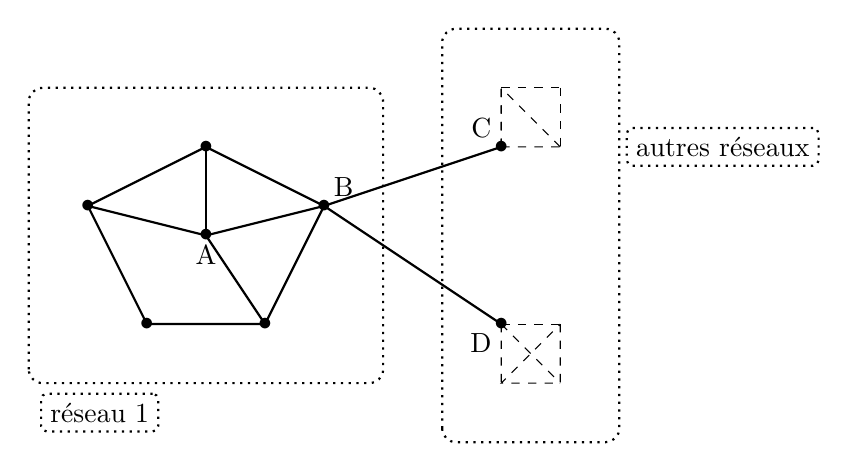
\begin{tikzpicture}[scale=0.75]
\coordinate (2) at (0,2);
\coordinate (3) at (1,0);
\coordinate (1) at (2,3);
\coordinate (4) at (3,0);
\coordinate (B) at (4,2);
\coordinate (A) at (2,1.5);
\coordinate (C) at (7,3);
\coordinate (D) at (7,0);

\draw (1) node{$\bullet$};
\draw (2) node{$\bullet$};
\draw (3) node{$\bullet$};
\draw (4) node{$\bullet$};
\draw (B) node[above right]{B} node{$\bullet$};
\draw (A) node[below]{A} node{$\bullet$};
\draw (C) node[above left]{C} node{$\bullet$};
\draw (D) node[below left]{D} node{$\bullet$};

\draw[thick] (1)--(2)--(3)--(4)--(B)--(1);
\draw[thick] (A)--(1);\draw[thick] (A)--(2);\draw[thick] (A)--(4);\draw[thick] (A)--(B);
\draw[thick] (B)--(C); \draw[thick] (B)--(D);
\draw[dashed] (C)--(7,4);\draw[dashed] (C)--(8,3);\draw[dashed] (C)--(7,4); \draw[dashed] (7,4)--(8,4);\draw[dashed] (8,4)--(8,3);\draw[dashed] (8,3)--(7,4);
\draw[dashed] (D)--(8,0);\draw[dashed] (D)--(8,-1);\draw[dashed] (D)--(7,-1);\draw[dashed] (8,0)--(8,-1)--(7,-1)--(8,0);

\draw[dotted, rounded corners=5pt, thick] (-1,-1) rectangle (5,4);
\node[draw,dotted, thick,rectangle, rounded corners=2pt] (R1) at (0.2,-1.5) {réseau 1};

\draw[dotted, rounded corners=5pt, thick] (6,-2) rectangle (9,5);
\node[draw,dotted, thick,rectangle, rounded corners=2pt] (R1) at (10.75,3) {autres réseaux};

\end{tikzpicture}
\caption{Un réseau central lié à deux autres sous-réseaux}
\label{graph:graphe1}
\end{figure}

On peut aussi apercevoir que le noeud \textbf{A}  est localisé là où le coefficient de regroupement est assez élevé contrairement à \textbf{B} qui est dans une zone à faible densité . On dit que les liens de \textbf{A} sont 'incrustés', ils ont un enchâssement significatif. 

Deux individus connectés par un lien possédant un grand enchâssement  auront une plus grande confiance mutuelle. En plus de la simple force du lien, c'est également la structure du réseau qui va augmenter la confiance entre deux nœuds. Il y aura une observation mutuelle, une surveillance de la part des amis communs aux deux nœuds.
Une représentation de ce concept est donnée dans le graphe ~\ref{graph:graphe2}. Dans cette figure, une observation mutuelle entre \textbf{A} et \textbf{B} est de mise.

\begin{figure}[h!]
\centering
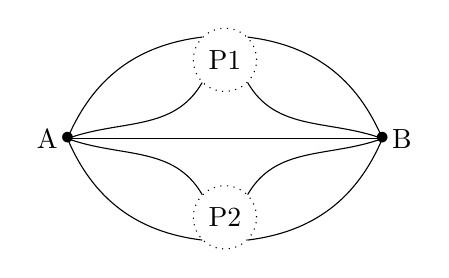
\begin{tikzpicture}
\coordinate (A) at (0,0);
\coordinate (B) at (4,0);


\draw (B) node[right]{B} node{$\bullet$};
\draw (A) node[left]{A} node{$\bullet$};
\node[draw,circle,dotted] (P1) at (2,1){P1};
\node[draw,circle,dotted] (P2) at (2,-1){P2};

\draw (A)--(B);

\draw (A) to[bend left] (P1.north west) (P1.north east) to[bend left](B);
\draw (A) edge[out=20, in=-120] (P1.south west) (P1.south east) edge[out=-60, in=160] (B);

\draw (A) edge[out=-20,in=120] (P2.north west) (P2.north east) edge[out=60,in=-160](B);
\draw (A) to[bend right]  (P2.south west) (P2.south east) to[bend right] (B);

\end{tikzpicture}
\caption{Deux noeuds possédant un enchâssement significatif}
\label{graph:graphe2}
\end{figure}

 En effet, imaginons que le noeud \textbf{A} effectue une action quelconque, tous les autres noeuds (par exemple, ceux de \textit{P1} et \textit{P2}) peuvent voir cette action.
Ainsi, deux noeuds possédant un enchâssement suffisamment conséquent ont une certaine confiance mutuelle.

On peut donc en tirer la propriété suivante provenant directement de la structure du graphe :

\vspace{1ex}
\textit{Plus l'enchâssement augmente, plus la confiance mutuelle est grande.}

\vspace{1ex}
En conséquence, \textbf{A} possède une grande influence car il a une forte confiance mutuelle avec tous ses amis.

Revenons maintenant au graphique \ref{graph:graphe1}. Bien que le lien \textbf{A} possède un grand enchâssement, il n'en est pas de même pour \textbf{B} avec \textbf{C} et \textbf{D}.
En effet, ils ne peuvent pas avoir une confiance mutuelle, car les autres noeuds de leur réseau respectif ne peuvent plus les "observer".

\vspace{1ex}
Bien que d'un certain point de vue, \textbf{A} pourrait posséder plus d'avantages que \textbf{B} grâce à ses fermetures et son voisinage, ce n'est pas tout à fait exact. Le noeud \textbf{B} possède lui aussi des avantages aussi fondamentaux que \textbf{A}.

\vspace{1ex}
\begin{itemize}
\item \textbf{B} est au bord d'un pont local. Il joue le rôle d'intermédiaire entre plusieurs réseaux.
\item \textbf{B} s'étend sur un trou structurel, il remplit le vide entre plusieurs ensembles de noeuds.
\item \textbf{B} est le seul lien pour communiquer avec certains ensembles. Tous les chemins entre ces deux communautés passent par \textbf{B}. Il est donc incontournable.
\item Il a des informations dispersées auxquelles les autres n'ont pas accès. Il va donc pouvoir amplifier sa créativité en observant les informations ou en en faisant passer certaines pour siennes.\footnote{Le fait d'être présent sur un pont pour pouvoir espionner efficacement peut par exemple être observé dans les programmes de surveillance des la NSA (États-Unis) ou du GCHQ (Grande-Bretagne) qui profitent du pont internet entre l'Europe et l'Amérique.}
\item Il joue le rôle de gardiennage social, il peut réguler l'accès de l'extérieur.
\end{itemize}

Par ailleurs, ces quelques derniers avantages peuvent engendrer un conflit d'intérêts entre \textbf{B} et ses sous-ensembles. Par exemple, dans le cas où \textbf{B} voudrait laisser deux réseaux scindés alors que ceux-ci désireraient s'assembler.\\

$\Rightarrow$ On fait donc appel à des notions de \textit{pouvoir} ou d'\textit{avantage}.\\

Ces notions sont aussi appelées \textit{capital social} ou capacité à se procurer des avantages grâce à l'appartenance à une structure sociale.

%Sur ce graphe distinguons les noeuds adjacents A et B.
%A: 
%- plus de confiance grâce à la fermeture dans son voisinage.
%
%B a d'autres avantages qui sont aussi fondamentaux:
%- B est au bord d'un pont local. Il joue le rôle d'intermédiaire entre plusieurs communautés.
%- B s'étend sur un trou structurel, il rempli le vide entre plusieurs ensembles de noeuds. 
%- B est le seul lien pour communiquer avec certains ensemble. En fait, tous les chemins entre ces deux %communautés passent par B. 
%- B a des informations dispersées auxquelles les autres n'ont pas accès. C'est un amplificateur de créativité.

\subsection{Notion de capital social}
Le capital social est la capacité à se procurer des avantages grâce à l'appartenance à une structure sociale. C'est une forme de capital, car elle représente une capacité que l'on possède et que l'on peut utiliser.  
Il existe d'autres notions de capitaux:\\

\begin{itemize}
\item Capital physique (exemple : technologie ) 
\item Capital humain (exemple : expertise des personnes )
\item Capital économique (exemple : monétaire ) 
\item Capital culturel (exemple : les ressources accumulées dans une culture, les connaissances communes )
\end{itemize}

\section{Similitude des noeuds}
Après nous être intéressés aux liens entre les noeuds, nous allons nous concentrer sur les similitudes entre  ces noeuds. 

\subsection{Principe de similitude}
La notion sociologique de similitude s'observe par une augmentation du nombre de liens entre les noeuds. 
Exemple: Les étudiants de l'UCL présentent une similitude par le fait qu'ils font partie de la même université. 

Ce principe implique de nouveaux mécanismes dans la manière où nous allons représenter les graphes:

\begin{tabular}{lcp{7cm}}
Sélection & $\longrightarrow$ & \textit{local} (Chacun choisi ses amis) \\
Influence sociale & $\longrightarrow$ & \textit{global/extérieur} (Induite par les gens que l'on fréquente)
\end{tabular}

Exemple de la propriété d'influence sociale :\\ Le fait d'être dans le même auditoire qu'un autre individu peut constituer un lien dans le graphe.

Bien que la sociologie est un concept difficile à formaliser. 
Une idée pourrait être d'inclure les facteurs de similitudes dans le graphe.

\begin{figure}[!h]
\centering
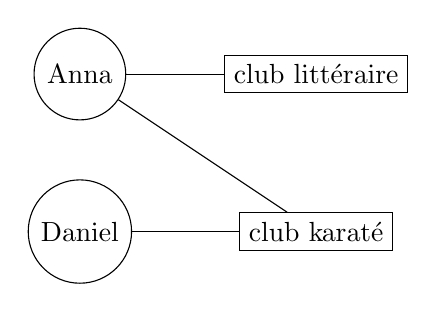
\begin{tikzpicture}
\coordinate (Dan) at (0,0);
\coordinate (An) at (0,2);
\coordinate (lit) at (3,2);
\coordinate (kar) at (3,0);


\node[draw,circle] (Dan) at (Dan){Daniel};
\node[draw,circle] (An) at (An){Anna};
\node[draw] (kar) at (kar){club karaté};
\node[draw] (lit) at (lit){club littéraire};

\draw  (An)--(lit);
\draw (An)--(kar);
\draw (Dan)--(kar);

\end{tikzpicture}
\caption{Exemple d'un graphe personnes-intérêts}

\label{graph:graphe3-1}
\end{figure}


Les graphes sont maintenant constitués à partir de deux types de noeuds:
\begin{itemize}
\item noeud Individu : représente une personne physique.
\item noeud Focus : activité ou centre d'intérêt.
\end{itemize}

Mais aussi de deux types de liens:
\begin{itemize}
\item liens Personnes - Personnes
\item liens Personnes - Focus
\end{itemize}

Ces graphes aussi appelés réseau d'affiliations ont une caractéristique bien particulière, ils sont toujours bipartis.

\vspace{1ex}
Définition \textit{graphe biparti}: Soit un graphe G=G(V,E) et $V_{1}$, $V_{2}$ deux ensembles de noeuds et $ V_{1} \cup V_{2} = V $, un graphe est dit biparti s'il n'existe pas d'arête interne dans ces deux sous-ensembles.\\ $ \forall e = (u,v)\in E, u \in V_{1}$ et $v \in V_{2} $.

\vspace{1ex}
Le graphe ci-dessous représente l'affiliation des personnes (A, B, C, D) au conseil d'administration de différentes entreprises.
Comme on peut le voir (graphe \ref{graph:grapheGoogle}), il peut y avoir un conflit d'intérêts, par exemple entre Google et Apple. En effet, les deux compagnies sont concurrentes (sur le marché des smartphones), et pourtant une personne est membre des deux conseils d'administration.

\begin{figure}[h!]
\centering
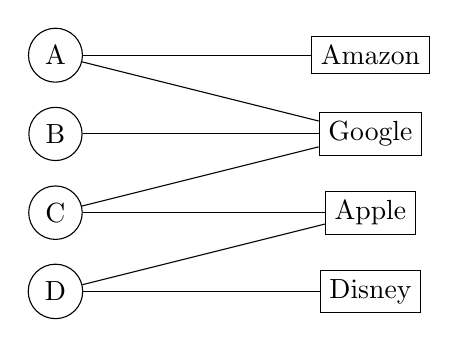
\begin{tikzpicture}
\coordinate (D) at (0,0);
\coordinate (C) at (0,1);
\coordinate (B) at (0,2);
\coordinate (A) at (0,3);

\coordinate (Dis) at (4,0);
\coordinate (Ap) at (4,1);
\coordinate (Go) at (4,2);
\coordinate (Am) at (4,3);

\node[draw,circle] (D) at (D){D};
\node[draw,circle] (C) at (C){C};
\node[draw,circle] (B) at (B){B};
\node[draw,circle] (A) at (A){A};

\node[draw] (Dis) at (Dis){Disney};
\node[draw] (Ap) at (Ap){Apple};
\node[draw] (Go) at (Go){Google};
\node[draw] (Am) at (Am){Amazon};

\draw (A)--(Am);
\draw (A)--(Go);
\draw (B)--(Go);
\draw (C)--(Go);
\draw (C)--(Ap);
\draw (D)--(Ap);
\draw (D)--(Dis);

\end{tikzpicture}
\caption{Exemple d'un graphe représentant un conseil d'administration}

\label{graph:grapheGoogle}
\end{figure}

Par ailleurs, ces graphes bipartis ne sont pas statiques. En effet, ils peuvent subir des évolutions dans le temps comme des ajouts de noeuds, points d'intérêts, nouveaux liens ...\\

Ainsi, ces graphes nous fournissent plus de précisions que les précédents. 
Grâce à ce concept, on peut voir plus efficacement les changements et transformations lors d'évolutions.

\subsection{Nouveaux mécanismes de fermeture}
Nous avons déjà vu précédemment le principe de fermeture triadique.\\

\begin{figure}[h!]
\centering
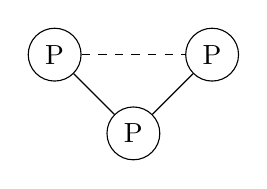
\begin{tikzpicture}
\coordinate (A) at (0,1);
\coordinate (B) at (1,0);
\coordinate (C) at (2,1);


\node[draw,circle] (A) at (A){P};
\node[draw,circle] (B) at (B){P};
\node[draw,circle] (C) at (C){P};

\draw  (A)--(B);
\draw [dashed] (A)--(C);
\draw (C)--(B);

\end{tikzpicture}
\caption{Rappel de fermeture triadique}

\label{graph:graphe3}
\end{figure}

Grâce à la prise en compte des points d'intérêts (focus), deux nouveaux principes de fermeture peuvent être considérés:

\subsubsection{Fermeture focale}
\begin{figure}[h!]
\centering
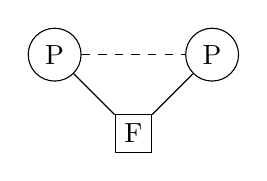
\begin{tikzpicture}
\coordinate (A) at (0,1);
\coordinate (B) at (1,0);
\coordinate (C) at (2,1);


\node[draw,circle] (A) at (A){P};
\node[draw] (B) at (B){F};
\node[draw,circle] (C) at (C){P};

\draw  (A)--(B);
\draw [dashed] (A)--(C);
\draw (C)--(B);

\end{tikzpicture}
\caption{Exemple de fermeture focale}

\label{graph:graphe3}
\end{figure}

Comme on peut le voir sur le graphique~\ref{graph:graphe3}, deux personnes ayant des similitudes ou mêmes centres d'intérêts, peuvent devenir amis.

\subsubsection{Fermeture d'adhésion}
De la même manière, une personne ayant une activité peut convertir son ami.
\begin{figure}[h!]
\centering
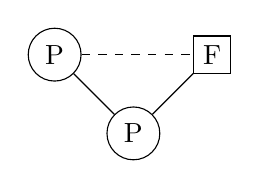
\begin{tikzpicture}
\coordinate (A) at (0,1);
\coordinate (B) at (1,0);
\coordinate (C) at (2,1);


\node[draw,circle] (A) at (A){P};
\node[draw,circle] (B) at (B){P};
\node[draw] (C) at (C){F};

\draw  (A)--(B);
\draw [dashed] (A)--(C);
\draw (C)--(B);

\end{tikzpicture}
\caption{Exemple de fermeture d'adhésion}
\label{graph:graphe4}
\end{figure}

Ces deux nouveaux mécanismes de fermeture permettent de raisonner beaucoup plus fort sur ces graphes. Ils sont même essentiels ! Si on ne les prenait pas en compte, on ne pourrait jamais comprendre pourquoi un lien apparaît spontanément.

\vspace{1ex}
Ci-dessous, un exemple illustrant cette propriété:

\vspace{1ex}
Sans les concepts introduits dans cette partie, voici ce que l'on observerait:

\begin{figure}[h!]
\centering
\begin{tabular}{ccc}
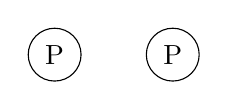
\begin{tikzpicture}
\coordinate (A) at (0,0);
\coordinate (C) at (1.5,0);

\node[draw,circle] (A) at (A){P};
\node[draw,circle] (C) at (C){P};

\end{tikzpicture}
& \raisebox{2ex}{$\qquad \longrightarrow \qquad$}
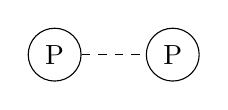
\begin{tikzpicture}
\coordinate (A) at (0,0);
\coordinate (C) at (1.5,0);

\node[draw,circle] (A) at (A){P};
\node[draw,circle] (C) at (C){P};
\draw[dashed] (A)--(C);

\end{tikzpicture}
\end{tabular}
\caption{Apparition spontanée d'un lien}
\label{graph:graphe5}
\end{figure}

Heureusement avec la propriété de fermeture focale, on peut raisonner sur la raison de cette apparition.

\begin{figure}[!h]
\centering
\begin{tabular}{ccc}
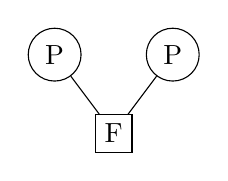
\begin{tikzpicture}
\coordinate (A) at (0,0);
\coordinate (B) at (0.75,-1);
\coordinate (C) at (1.5,0);

\node[draw,circle] (A) at (A){P};
\node[draw] (B) at (B){F};
\node[draw,circle] (C) at (C){P};
\draw (B)--(A);
\draw (B)--(C);
\end{tikzpicture}
& \raisebox{4ex}{$\qquad \longrightarrow \qquad$}
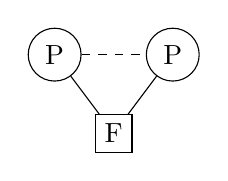
\begin{tikzpicture}
\coordinate (A) at (0,0);
\coordinate (B) at (0.75,-1);
\coordinate (C) at (1.5,0);

\node[draw,circle] (A) at (A){P};
\node[draw] (B) at (B){F};
\node[draw,circle] (C) at (C){P};
\draw (B)--(A);
\draw (B)--(C);
\draw[dashed] (A)--(C);
\end{tikzpicture}
\end{tabular}
\caption{Apparition du lien dû au focus en commun}
\label{graph:graphe5}
\end{figure}

\subsection*{Coefficient de regroupement}
Le coefficient de regroupement ou en anglais, \textit{clustering coefficient}, représente la probabilité pour un nœud \textbf{A} que deux amis de celui-ci choisi aléatoirement, soit amis entre eux. 
$$ \text{Clustering coefficient} = \frac{\text{nombre d'arêtes existantes reliant les amis de \textbf{A}}}{\text{nombre total d'arêtes possible reliant les amis de \textbf{A}}}$$

Un exemple de ce concept est donné pour la figure suivante.

\begin{figure}[h!]
\centering
\includegraphics[scale=0.8]{images/20_img1.png}
\caption{Graphe simple}
\label{img:coef-regr-exp}
\end{figure}

Considérons la figure \ref{img:coef-regr-exp}. Le coefficient de regroupement pour le nœud \textbf{A} est $,\frac{1}{6}$ car il n'y a qu'une seule arête (\textbf{C-D}) parmi les six autres paires possibles (\textbf{B-C}, \textbf{B-D}, \textbf{B-E}, \textbf{C-D}, \textbf{C-E}, et \textbf{D-E}) reliées entre elles.
